\documentclass{article}
\usepackage[utf8]{inputenc}
\usepackage{geometry}
\usepackage{url}
\usepackage[utopia]{mathdesign}
\usepackage{amsmath}
 \geometry{
 a4paper,
 total={170mm,257mm},
 left=20mm,
 top=20mm,
 }
\usepackage{graphicx}
\usepackage{tikz}
\usepackage{titling}
\usepackage{kinematikz}
 \title{2rd report of Advanced Topics in Robot Mechanism}
\author{GU JUN}
\date{Jan 15. 2025}
 
 \usepackage{fancyhdr}
\fancypagestyle{plain}{%  the preset of fancyhdr 
    \fancyhf{} % clear all header and footer fields
    \fancyfoot[R]{\thepage}
    \fancyfoot[L]{\theauthor}
    \fancyhead[L]{2024 Advanced Topics in Robot Mechanism}
    \fancyhead[R]{\thedate}
}
\makeatletter
\def\@maketitle{%
  \newpage
  \null
  \vskip 1em%
  \begin{center}%
  \let \footnote \thanks
    {\LARGE \@title \par}%
    \vskip 1em%
    %{\large \@date}%
  \end{center}%
  \par
  \vskip 1em}
\makeatother

\usepackage{lipsum}  
\usepackage{cmbright}
\begin{document}

\maketitle

\noindent\begin{tabular}{@{}ll}
    Student & \theauthor\\
    Student ID & 61322300564 \\
    Date & \thedate\\
\end{tabular}

% Among the robots that are eagerly awaited for development, design a robot in
% which the robot mechanism plays an important role, and draw a punch picture
% (handwritten with supplementary explanations to accompany the picture)
% using technical illustration techniques that clearly shows the main points of the
% robot mechanism.
\section*{A wheel-legged robot with 7 DOF}

A bipedal wheel-legged robot is a hybrid robotic system that combines the advantages of both wheels and legs to achieve versatile and efficient locomotion. 
This type of robot is designed to navigate a variety of terrains by leveraging the agility of legged locomotion and the efficiency of wheeled movement.\cite{bjelonic2019keep}
The wheel-legged design allows the robot to switch between rolling on smooth surfaces and walking or climbing or even jumping on rough or uneven terrain.\cite{klemm2019ascento} 
This dual capability enhances the robot's adaptability, making it suitable for tasks in diverse environments, such as urban search and rescue, exploration, and service robotics.\cite{li2023design}
The legs provide the robot with the ability to step over obstacles, climb stairs, and maintain stability on uneven ground. 

The wheels, on the other hand, enable fast and energy-efficient travel on flat surfaces. 
By integrating both mechanisms, the bipedal wheel-legged robot can perform complex maneuvers that are challenging for traditional wheeled or legged robots alone.
In summary, a bipedal wheel-legged robot offers a promising solution for applications requiring both agility and efficiency in locomotion, combining the best features of wheels and legs to navigate a wide range of environments effectively.

\begin{figure}[h!]
  \centering
  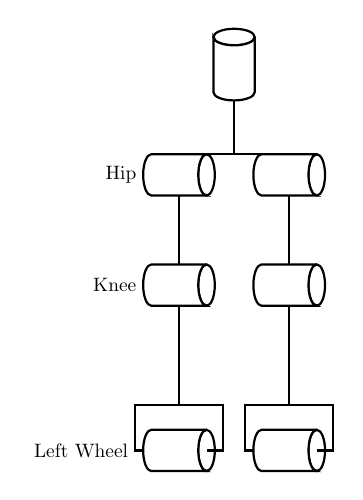
\begin{tikzpicture}[scale=0.7,transform shape]
  \pic (left_wheel) at (0, 0) {rotational 3D H=1};
  \node [left] at (left_wheel-west) {Left Wheel};
  \pic (J1) at (0, 3) {rotational 3D H=0};
  \node [left] at (J1-west) {Knee};
  \pic (J2) at (0, 5) {rotational 3D H=0};
  \node [left] at (J2-west) {Hip};
  \pic (J3) at (1, 7) {rotational 3D V=0};
  \pic (right_wheel) at (2, 0) {rotational 3D H=1};
  \pic (J4) at (2, 3) {rotational 3D H=0};
  \pic (J5) at (2, 5) {rotational 3D H=0};
  \draw [knLinkStyle]
  (left_wheel-out) -- (J1-south)
  (J1-north) -- (J2-south)
  (J2-north) -| (J3-south);
  \draw [knLinkStyle]
  (right_wheel-out) -- (J4-south)
  (J4-north) -- (J5-south)
  (J5-north) -| (J3-south);
  \end{tikzpicture}
  \caption{\textbf{A wheel-legged robot with 7 DOF.} The robot has two legs and two wheels as feet. 
  Each leg has 3 DOF, and the body has 1 DOF. The wheels are actuated by a separate motor.}
    \label{fig:wheel-legged-robot}
\end{figure}

% Explain in detail the function and performance of the robot in the text.
%  (*) All the text should be written in Word or LaTeX, except for the punch
% drawing.

Here is the description of the robot's function and performance. As you can see in the figure.\ref{fig:wheel-legged-robot}, 
the robot has two legs and two wheels as feet. Each leg has 3 DOF, and the body has 1 DOF. For one leg, there are hip and knee joints, the robot can use them to keep balance, climb stairs, and even jump.

I also add a DOF to the body of the robot, which is useful for adjusting the CoM of the robot, and can be used for balance control and further upper body posture adjustment.

The wheels are actuated by a separate motor, which allows the robot to switch between rolling and walking modes. The robot can roll on flat surfaces using the wheels, and walk or climb using the legs. This dual-mode locomotion enables the robot to navigate a wide range of terrains efficiently and effectively.
The legs can also benefit the rolling mode by providing additional stability and traction when needed. This hybrid locomotion system combines the advantages of wheeled and legged robots, 
making the robot versatile and adaptable to various environments and tasks. This robot can be used in applications such as search and rescue, exploration, and service robotics, where agility and efficiency in locomotion are essential.
\newpage

\section*{Technology analysis of the robot}

% For the robot designed in (1), explain in details the structure and properties
% of the robot mechanism related to the assumed functions and performance
% from a technical point of view using knowledge and methods of robot
% mechanics in the form of academic paper. The whole or a part of the designed
% robot mechanism should be used in the paper.

In this section, I will analyze the structure and properties of the wheel-legged robot designed in the previous section from a technical point of view.
To achieve the locomotion capabilities of the robot, we need to consider the popular walking control algorithms, such as ZMP-based control, LQR control, and reinforcement learning-based control.
Whatever the control algorithm is, we need to drive the reaction forces and the position of the feet to achieve the desired motion. 
And the kinematic and dynamic analysis of the robot is essential for the control algorithm.

Because two legs have the same structure, I will analyze one leg of the robot. And the wheel is actuated by a separate motor, which is not the focus of this analysis.
So in this section, I will focus on the kinematic and dynamic analysis of a simplified version of the leg, which has 2 DOF.

%TODO: Figure of the simplified leg with 2 DOF
\begin{figure}[h!]
  \centering
  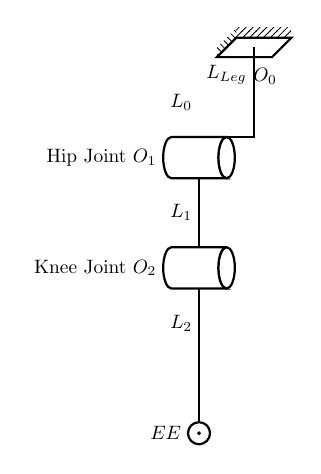
\begin{tikzpicture}[scale=0.7,transform shape]
  \pic (left_wheel) at (0, 0) {cylindrical pair F};
  \node [left] at (-0.2, 0) {$EE$};
  \pic (J1) at (0, 3) {rotational 3D H=0};
  \node [left] at (J1-west) {Knee Joint $O_2$};
  \node [left] at (0, 2) {$L_2$};
  \pic (J2) at (0, 5) {rotational 3D H=0};
  \node [left] at (J2-west) {Hip Joint $O_1$};
  \node [left] at (0, 4) {$L_1$};
  \pic [rotate=180] (J3) at (1, 7) {frame 3D};
  \node [above] at (1.2, 6.2) {$O_0$};
  \node [left] at (0, 6) {$L_0$};
  \node [] at (0.5, 6.5) {$L_{Leg}$};
  \draw [knLinkStyle]
  (left_wheel-out) -- (J1-south)
  (J1-north) -- (J2-south)
  (J2-north) -| (J3-center);
  \end{tikzpicture}
  \caption{\textbf{The simplified left leg kinematic model} Where $L_0$ is the length of the body, $L_1$ is the length of the thigh, 
          and $L_2$ is the length of the calf. $L_{Leg}$ is the distance between leg and body.}
    \label{fig:left-leg}
\end{figure}



After defining the coordinates of the leg, we can use the DH parameters to define the structure of the leg. The DH parameters are shown in Table \ref{tab:dh_parameters}.
\begin{table}[h!]
  \centering
  \small
  \begin{tabular}{|c|c|c|c|c|}
  \hline
  Joint & $a_{i-1}$ & $\alpha_{i-1}$ & $d_i$ & $\theta_i$ \\
  \hline
  Hip & $L_{Leg}$ & $\frac{\pi}{2}$ & $L_{0}$ & $\theta_1$ \\
  Knee & $L_1$ & 0 & $0$ & $\theta_2$ \\
  EE & $L_2$ & $-\frac{\pi}{2}$ & $0$ & 0 \\
  \hline
  \end{tabular}
  \caption{DH Parameters for the simplified leg}
  \label{tab:dh_parameters}
\end{table}
  
\section*{Kinematic Equation Derivation}
The transformation matrix for each joint using DH parameters is given by:

\begin{equation}
  { }^{n-1} T_n=\left[\begin{smallmatrix}
  \cos \theta_n & -\sin \theta_n & 0 & a_{n-1} \\
  \sin \theta_n \cos \alpha_{n-1} & \cos \theta_n \cos \alpha_{n-1} & -\sin \alpha_{n-1} & -d_n \sin \alpha_{n-1} \\
  \sin \theta_n \sin \alpha_{n-1} & \cos \theta_n \sin \alpha_{n-1} & \cos \alpha_{n-1} & d_n \cos \alpha_{n-1} \\
  0 & 0 & 0 & 1
  \end{smallmatrix}\right]
\end{equation}

With the transformation matrix for each joint, we can derive the forward kinematics equation for the leg.
The forward kinematics equation is given by:
\begin{equation}
  T_{0}^{3}=T_{0}^{1} T_{1}^{2} T_{2}^{3}
  \end{equation}
  where $T_{0}^{1}$, $T_{1}^{2}$, and $T_{2}^{3}$ are the transformation matrices for the hip, knee, and end effector joints, respectively.
  By multiplying the transformation matrices, we can derive the forward kinematics equation for the leg.
And the result is:
\begin{equation}
  T_{0}^{3}=\left[\begin{smallmatrix}
  \cos (\theta_1 - \theta_2) & 0 & -\sin (\theta_1 + \theta_2) & L_2 \cos (\theta_1 - \theta_2) + L_1 \cos \theta_1 + L_{Leg} \\
  0 & 0 & 0 & -L_0 \\
  \sin(\theta_1 - \theta_2) & 0 & \cos (\theta_1 - \theta_2) & L_2 \sin (\theta_1 - \theta_2) + L_1 \sin \theta_1 \\
  0 & 0 & 0 & 1
  \end{smallmatrix}\right]
\end{equation}

With the forward kinematics equation, we can calculate the position and orientation of the end effector of the leg given the joint angles. 
We also can derive the Jacobian matrix for the leg to analyze the velocity and acceleration of the end effector. And further use it for the dynamic analysis of the leg.
I will skip the derivation of the Jacobian matrix and dynamic analysis in this report.
Further, I modeled the robot in a simulation environment called Isaac-sim and use the reinforcement learning algorithm to control the robot to keep balance and roll on the ground.

\section*{Simulation in Isaac-sim and Reinforcement Learning Control}
Recently reinforcement learning\cite{kaelbling1996reinforcement} has been widely used in robotics to solve complex control problems.\cite{hoeller2024anymal} Although we have the kinematic and dynamic model of the robot, 
it is still challenging to derive an analytical solution for the control problem. So I use the reinforcement learning algorithm to control the robot to keep balance and roll on the ground.
And I use the Isaac-sim as the simulation environment to train the robot.\cite{web:isaac-sim}\cite{mittal2023orbit} The Isaac-sim is a high-fidelity simulation environment that provides realistic physics simulation and rendering capabilities provided by Nvidia.
It is very popular in the robotics community for training robots in a simulated environment before deploying them in the real world.\cite{kumar2021workflow}

I use the reinforcement learning algorithm called Proximal Policy Optimization (PPO) to train the robot to keep balance and roll on the ground. PPO is a state-of-the-art reinforcement learning algorithm that has been shown to be effective in solving complex control problems.\cite{thompson2019reinforcement}
\begin{figure}[h!]
  \centering
  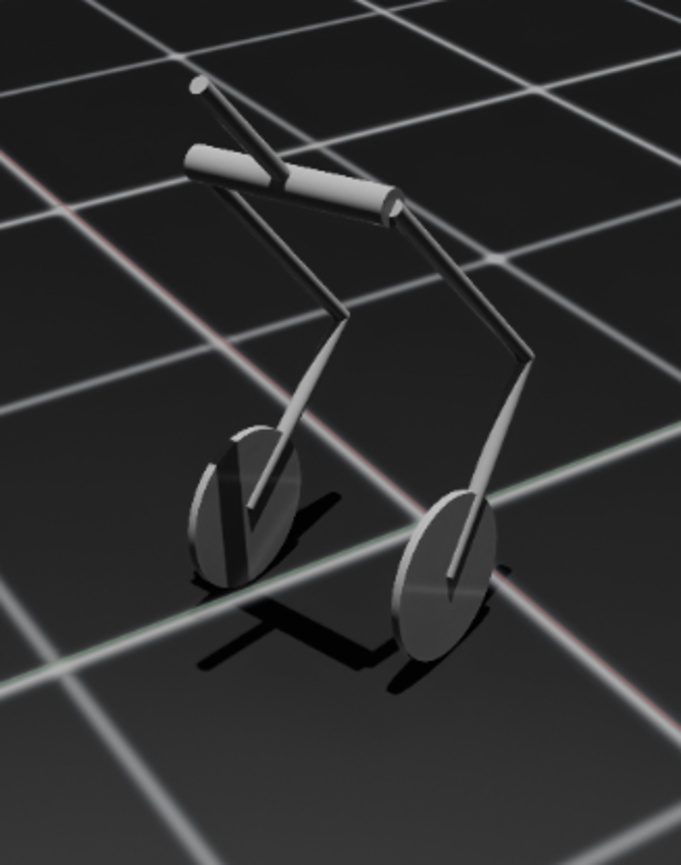
\includegraphics[height=0.5\textwidth]{assets/kinematic_model.pdf}
  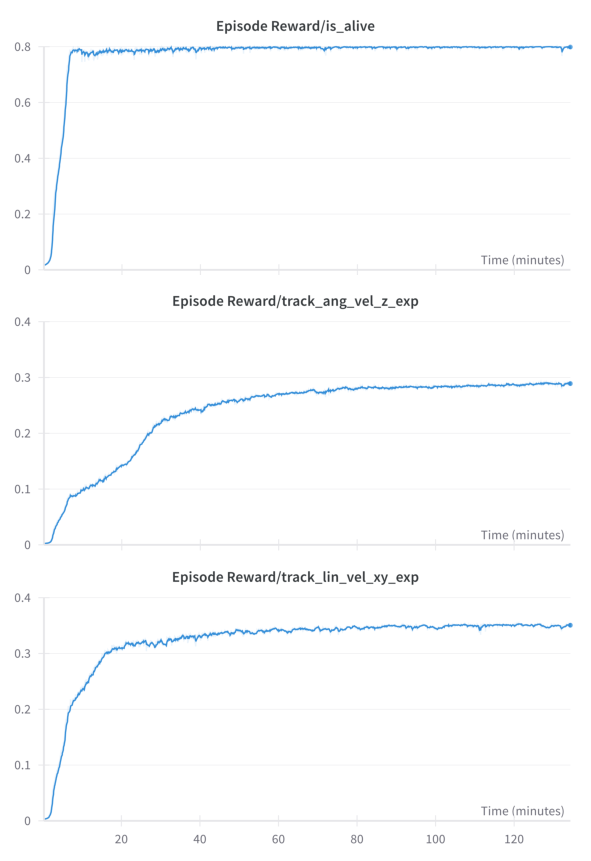
\includegraphics[height=0.5\textwidth]{assets/rewards.pdf}
  \caption{\textbf{The kinematic model of the robot in Isaac-sim(left), and the training result(right)} The robot has two legs and two wheels. After two hours of training, the robot can keep balance and follow the move commands.}
    \label{fig:isaac-sim}
\end{figure}

The training process is shown in the figure.\ref{fig:isaac-sim}. I will not go into detail about the reinforcement training process and in this report. 
But the result shows that the robot can keep balance and follow the move commands after two hours of training. This demonstrates the effectiveness of the reinforcement learning algorithm in controlling the robot to achieve the desired locomotion capabilities.
However, as a black box model, the reinforcement learning algorithm lacks interpretability and generalization capabilities. The trained model may be unstable or fail to generalize to unseen environments. 
Maybe in the future, we can combine the analytical model and the reinforcement learning algorithm to achieve better control performance.

\begin{figure}
  \centering
    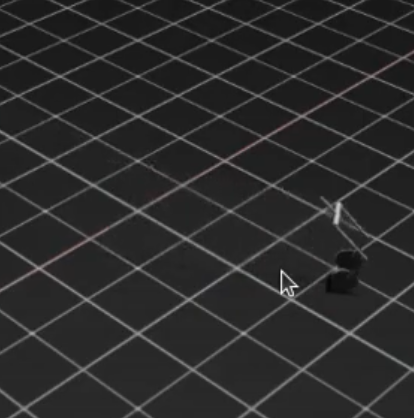
\includegraphics[width=0.22\textwidth]{assets/g1w_1.png}
    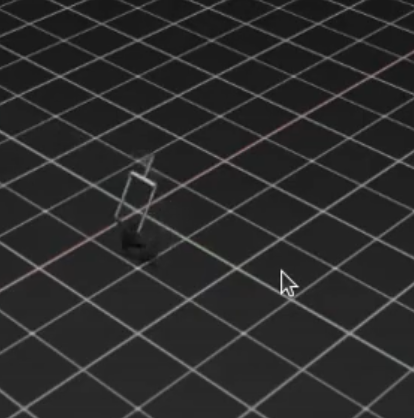
\includegraphics[width=0.22\textwidth]{assets/g1w_2.png}
    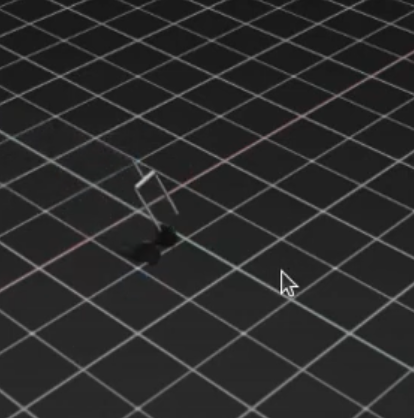
\includegraphics[width=0.22\textwidth]{assets/g1w_3.png}
    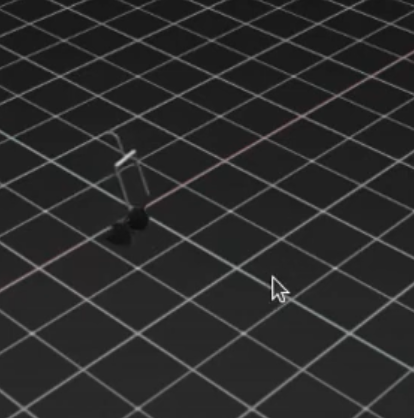
\includegraphics[width=0.22\textwidth]{assets/g1w_4.png}
  \caption{\textbf{Screenshots of the trained robot moving on the ground.} The robot can keep balance, go forward and backward, and turn left and right.\cite{web:g1w_move}}
    \label{fig:robot_movement}
\end{figure}

\newpage

\section*{Conclusion}
In this report, I presented a design of a wheel-legged robot with 7 DOF that combines the advantages of wheeled and legged locomotion to achieve versatile and efficient locomotion capabilities.
Further, I analyzed the kinematic properties of the robot from a technical point of view and used the Isaac-sim simulation environment to train the robot using the reinforcement learning algorithm.

In fact, this is part of my research project since last year. The robot is called G1W from our lab, and I am responsible for the reinforcement learning part of the project.
The result shows that the robot can keep balance and follow the move commands after two hours of training. 
This does inspire me to further explore the combination of analytical models and reinforcement learning algorithms to achieve better control performance in the future.

I do thank the professor for teaching us different method and knowledge about robot mechanism in details, which helps me a lot in my research project.

In the further research, I will focus on how to combine the analytical model and the reinforcement learning algorithm to achieve better control performance. 
Like not only use the general reinforcement learning algorithm but also use the model-based reinforcement learning algorithm to improve the control performance of the robot.
What's more, according to the features of the robot mechanism, maybe different deep network structures can be used to improve the training efficiency and performance of the robot.

\bibliographystyle{IEEEtran}
\bibliography{bibs/IEEEabrv, bibs/cites}

\end{document}
